%!tex root = ../main.tex

\section{Unsolvability in the PN Model} \label{sec:algorithm}

In this section, we will introduce the basic idea of an algorithm that finds a proof that an LCL problem is impossible to solve in the PN model.
If the algorithm detects the problem is unsolvable, it outputs a multigraph as a result.
In Sections~\ref{sec:algorithm:from_multiple_to_simple} and \ref{sec:algorithm:from_finite_to_infinite}, we show that this multigraph is a proof that the problem is unsolvable in the PN model.
In Section \ref{sec:algorithm:from_pn_to_local}, we prove that if an LCL problem is unsolvable in the PN model, then the problem is not solvable in constant time in the LOCAL model.

% In Section \ref{sec:algorithm:from_multiple_to_simple} we show that the unsolvability of a problem in finite PN networks with multiple connections implies the unsolvability of the problem in finite simple PN networks.
% Later in Section \ref{sec:algorithm:from_finite_to_infinite}, we show that the unsolvability of the problem in finite PN networks implies the unsolvability of the problem in infinite tree PN networks.
% Finally, in Section \ref{sec:algorithm:from_pn_to_local}, we show that the unsolvability of the problem in infinite tree PN networks implies the problem is not solvable in constant time in the LOCAL model.
%
We first formally define the meaning of solvability of an LCL problem in the PN model.
\begin{definition} \label{def:lcl_solvability}
    An LCL problem $\Pi$ is solvable in PN model, if and only if there exists a PN algorithm $A$ that finds a solution for $\Pi$ in all PN networks.
\end{definition}

We can define an alternative version of the Definition \ref{def:lcl_solvability} using contraposition.
\begin{corollary} \label{cor:lcl_solvability:contrapositive}
An LCL problem $\Pi$ is not solvable in PN model, if and only if there does not exist a PN algorithm $A$ that finds a solution for $\Pi$ in all PN networks.
\end{corollary}

We have illustrated two examples of unsolvable LCL problems in Tables \ref{tbl:unsolvable_lcl:1} and \ref{tbl:unsolvable_lcl:2}, where the values Y (Yes) and N (No) answer to the question: \emph{can the algorithm in this row solve the problem in the network of this column?}
Value of Y/N indicates that the value does not matter for the purpose of the example.
In both examples, there are only a finite number of networks and algorithms for the sake of simplicity.
In Table \ref{tbl:unsolvable_lcl:1}, the problem $\Pi$ is unsolvable, because there is at least one network for each algorithm, where the algorithm fails to solve the problem.
In Table \ref{tbl:unsolvable_lcl:2}, we show an example that is a special case of Corollary \ref{cor:lcl_solvability:contrapositive}.
The problem $\Pi'$ is also unsolvable, but this time no algorithm can solve it in network $N'_{n'}$.

\begin{table}[H]
    \parbox{.45\linewidth}{
    \centering
    \resizebox{0.45\textwidth}{!}{%
        \begin{tabular}{c|ccccc}
        $\Pi$&$N_1$&$N_2$&$N_3$&$\cdots$&$N_n$ \\
        \hline
        $A_1$& N & Y/N & Y/N & $\cdots$ &  Y/N  \\
        $A_2$& Y/N & N & Y/N & $\cdots$ &  Y/N  \\
        $A_3$& Y/N & Y/N & N& $\cdots$ &  Y/N  \\
        $\vdots$&$\vdots$&$\vdots$&$\vdots$&$\ddots$&$\vdots$ \\
        $A_{m}$& Y/N & Y/N & Y/N & $\cdots$ &  N \\
        \hline
        \end{tabular}
    }
    \caption{
        Unsolvable LCL problem $\Pi$.
        Each algorithm fails to solve $\Pi$ in at least some network, denoted by ``N'' (No).
    }
    \label{tbl:unsolvable_lcl:1}
    }
    \hfill
    \parbox{.45\linewidth}{
        \centering
    \resizebox{0.45\textwidth}{!}{%
        \begin{tabular}{c|ccccc}
        $\Pi'$&$N'_1$&$N'_2$&$N'_3$&$\cdots$&$N'_{n'}$ \\
        \hline
        $A'_1$& Y/N & Y/N & Y/N & $\cdots$ &  N \\
        $A'_2$& Y/N & Y/N & Y/N & $\cdots$ &  N \\
        $A'_3$& Y/N & Y/N & Y/N & $\cdots$ &  N \\
        $\vdots$&$\vdots$&$\vdots$&$\vdots$&$\ddots$&$\vdots$ \\
        $A'_{m'}$& Y/N & Y/N & Y/N & $\cdots$ &  N \\
        \hline
        \end{tabular}
    }
    \caption{
        Unsolvable LCL problem $\Pi'$.
        Each algorithm fails to solve $\Pi'$ at least in network $N'_{n'}$ (the last column containing only values ``N'').
    }
    \label{tbl:unsolvable_lcl:2}
    }
\end{table}

Not every unsolvable LCL problem necessarily fall within the case shown in Table~\ref{tbl:unsolvable_lcl:2}.
Nevertheless, we are interested in it, because it seems more feasible to find a single network where all algorithms fail, in comparison to finding a network for each algorithm separately.
The special case is written as follows.

\begin{lemma} \label{lem:lcl_unsolvability}
    An LCL problem $\Pi$ is not solvable in PN model, if there exists a PN network $N$ such that no PN algorithm $A$ can solve the problem $\Pi$ in network $N$.
\end{lemma}
\begin{proof}
    Let $\Pi$ be an LCL problem.
    Let $N$ be a PN network such that no PN algorithm $A$ can solve $\Pi$ in $N$.
    Therefore, no PN algorithm $A$ can find a solution to $\Pi$ in all PN networks.
    According to Corollary \ref{cor:lcl_solvability:contrapositive}, the problem $\Pi$ is unsolvable.
\end{proof}

From Lemma \ref{lem:lcl_unsolvability} we can say that, to show that a problem $\Pi$ is unsolvable in the PN model, it is sufficient to find a counterexample---a PN network $N$ in which the problem $\Pi$ cannot be solved.
We also show that a problem is not solvable in a PN network if it is not solvable in the underlying graph represented by the network.

\begin{lemma} \label{lem:problem_unsolvability_in_graphs}
    If a problem $\Pi$ is not solvable in graph $G$, then $\Pi$ is also not solvable in any PN network $N$ that has $G$ as its underlying graph.
\end{lemma}
\begin{proof}
    Let us assume that a problem $\Pi$ is not solvable in graph $G$, and $\Pi$ is solvable in some PN network $N$ that has $G$ as its underlying graph.
    This means that network $N$ has a valid labeling, thus its underlying graph $G$ has also a valid labeling.
    This is a contradiction, therefore the original implication must be true.
\end{proof}

With the fact from Lemma \ref{lem:problem_unsolvability_in_graphs}, we create an algorithm that automatically tries to find a counterexample---a graph for which the given LCL problem is not solvable.
The algorithm is written as follows.

\begin{algorithm}[H]
    \caption{Counterexample graph finder}
    \label{alg:counterexample_finder}
    \begin{algorithmic}[1] % The number tells where the line numbering should start
        \Require $1 \leq n_{low} \leq n_{high}$
        \Function{Find}{$n_{low},n_{high}, \Pi$} \Comment{Graph bounds $n_{low}$ and $n_{high}$, LCL problem $\Pi$} \label{alg:counterexample_finder:n_loop}
            \State $\Delta \gets \textsc{ActiveDegree}(\Pi)$ \label{alg:counterexample_finder:d_a}
            \State $\delta \gets \textsc{PassiveDegree}(\Pi)$ \label{alg:counterexample_finder:d_p}
            \For{$n\gets n_{low}, n_{high}$} \Comment{Iterate graph sizes from lowest to highest} \label{alg:counterexample_finder:n}
                \State $G_n \gets \textsc{GenerateGraphs}(n, \Delta, \delta)$ \label{alg:counterexample_finder:Gn}
                \ForEach{$g \in G_n$} \label{alg:counterexample_finder:g}
                    \If {\Not $\textsc{SolutionExists}(\Pi, g)$} \label{alg:counterexample_finder:solution_exists}
                        \State \Return $g$ \Comment{Return counterexample.}\label{alg:counterexample_finder:return_g}
                    \EndIf
                \EndFor
            \EndFor
            \State \Return \Comment{No counterexample found. Return nothing.} \label{alg:counterexample_finder:return_nothing}
        \EndFunction
    \end{algorithmic}
\end{algorithm}

The Algorithm \ref{alg:counterexample_finder} is designed to find the smallest graph for which an LCL problem $\Pi$ is not solvable.
It starts from graphs with $n_{low}$ vertices and goes up to graphs with $n_{high}$ vertices.
We define $\Delta$ and $\delta$ to be the active and passive degree of the problem $\Pi$ respectively (rows \ref{alg:counterexample_finder:d_a} and \ref{alg:counterexample_finder:d_p}).
The variable for the current vertex count is called $n$ (row~\ref{alg:counterexample_finder:n}).
For each $n$, we generate all possible $(\Delta, \delta)$-biregular multigraphs with $\textsc{GenerateGraphs}(n, \Delta, \delta)$, and save the multigraphs into variable $G_n$ (row~\ref{alg:counterexample_finder:Gn}).
%The reason for generating only these types of multigraphs comes from the LCL formalism from Section \ref{sec:lcl_problems:biregular}.
Now, for each multigraph $g \in G_n$ (row~\ref{alg:counterexample_finder:g}) we check if the given problem $\Pi$ has a solution using the function $\textsc{SolutionExists}(\Pi, g)$ (row~\ref{alg:counterexample_finder:solution_exists}).
If a solution does not exist, we return the multigraph as a counterexample (row~\ref{alg:counterexample_finder:return_g}).
In the case there are no counterexamples in multigraphs between $n_{low}$ and $n_{high}$ vertices, the algorithm returns nothing (row~\ref{alg:counterexample_finder:return_nothing}).

Up to this moment, we have not discussed how the function \[ \textsc{GenerateGraphs}(n, \Delta, \delta) \] from row~\ref{alg:counterexample_finder:Gn} actually generates the multigraphs, nor have we discussed how the function \[ \textsc{SolutionExists}(\Pi, g) \] from row~\ref{alg:counterexample_finder:solution_exists} determines the existence of a solution.
These functions are implementation specific and in this section we assume that they exist as black boxes.
We discuss our implementations of these functions later in Section~\ref{sec:implementation}.
However, we can discuss why the algorithm generates multigraphs instead of simple graphs.
The algorithm generates multigraphs, because they are less restrictive than simple graphs.
Thus, we generate more graphs when multiple edges are allowed, which implies more possibilities to find a counterexample.

As we said before, we use the LCL formalism from Section \ref{sec:lcl_problems:biregular}.
The formalism uses infinite $(\Delta, \delta)$-biregular trees, but the algorithm generates finite $(\Delta, \delta)$-biregular multigraphs.
In Section~\ref{sec:algorithm:from_multiple_to_simple}, we show if we can find $(\Delta, \delta)$-biregular network with multiple connections, where the problem is unsolvable, then it implies that it is also unsolvable in some simple $(\Delta, \delta)$-biregular network.
This can be derived to work with graphs with Lemma~\ref{lem:problem_unsolvability_in_graphs}.
In Section~\ref{sec:algorithm:from_finite_to_infinite}, we show that if an LCL problem is unsolvable in finite connected $(\Delta, \delta)$-biregular graph $G$ with cycles, then it is also unsolvable in some infinite $(\Delta, \delta)$-biregular tree $G'$.
Finite $(\Delta, \delta)$-biregular graphs are always with cycles, when both $\Delta$ and $\delta$ are greater than 1, and this is in practice always the case, because we are not interested in biregular graphs with $\Delta=1$ or $\delta=1$ as they are trivial.


\subsection{From Multiple Connection Networks to Simple Networks} \label{sec:algorithm:from_multiple_to_simple}

In this section we show that if an LCL problem is not solvable in PN networks with multiple connections, then the problem is also not solvable in simple PN networks.

% Pi is unsolvable in multiple connection PN network N -> Pi is unsolvable in lift of N
\begin{lemma} \label{lem:lcl_unsolvability:from_multiple_to_lift}
If an LCL problem $\Pi$ is not solvable in a PN network $N$, then it is also not solvable in any PN network $N'$ that is a lift of $N$.
\end{lemma}
\begin{proof}
    Since problem $\Pi$ has no solution in some PN network $N$, any algorithm $A$ will produce an invalid solution to $\Pi$ i.e.\ a local constraint is violated at least at some node $v$.
    Let $\phi: V' \rightarrow V$ be a covering map from $N'=(V', P', p')$ to $N=(V, P, p)$.
    Theorem 7.1 from the textbook \cite{HirvonenSuomelaDistAlg2020} shows that the nodes of $N'$ will have exactly the same state as their counterparts at $N$ for each time unit $t=0,1,...$\;.
    Hence, if we run algorithm $A$ on both networks $N$ and $N'$, the local constraint violation at some node $v \in N$ also appears in all nodes $v' \in V'$ such that $\phi(v') = v$ i.e.\ the local constraint violations also appear in the covering network $N'$.
\end{proof}

% Network with multiple connections ----k-lift--->  simple network
\begin{lemma} \label{lem:lcl_unsolvability:from_klift_to_simple}
    If there is a PN network $N_2$ with at most $k$ connections between any two nodes, then there exists a $k$-lift $N_1$ of $N_2$ such that $N_1$ is a simple PN network.
\end{lemma}
\begin{proof}
    Let $N_2=(V_2, P_2, p_2)$, and $\operatorname{mul}(u, v)$ be the number of connections between any nodes $u, v \in V_2$.
    Thus, we can say that $k = \max (\{ m(u, v) \mid u, v \in V_2\} )$.
    Let $\operatorname{M}: \mathbb{N}_{> 0} \rightarrow \{1, ..., k\}$ be a function defined as $\operatorname{M}(x+hk) = x$ for all $x = 1, ..., k$ and $h\in \mathbb{N}$.
    For example $\operatorname{M}(1 + hk) = 1$ and $\operatorname{M}(k + hk) = k$.

    Let $N_1=(V_1, P_1, p_1)$ be another network such that:
    \begin{itemize}
        \item For each $v \in V_2$, there are $k$ copies in $V_1$, namely $v_1, v_2, ..., v_k \in V_1$.
        Thus, the sizes $|V_1|$ and $k|V_2|$ are equal.
        \item For each port $(v, i) \in P_2$, we have ports $(v_x, i) \in P_1$ where $x=1, 2, ..., k$.
        \item For each multiple connection $p_2((v, i_a)) = (u, j_a)$ where $a = 1, 2, ..., \operatorname{mul}(u, v)$, we have $p_1((v_{x}, i_a)) = (u_{\operatorname{M}(x+a-1)}, j_a)$.
        Here $i_a$ is $a$-th port number of $v$ that connects to $u$, and $j_a$ is $a$-th port number of $u$ that connects to $v$.
        Note that if $\operatorname{mul}(u, v) = 1$, then $p_1((v_{x}, i_1)) = (u_{\operatorname{M}(x)}, j_1) = (u_{x}, j_1)$.
    \end{itemize}

    Now we show that there is a covering map $\phi: V_1 \rightarrow V_2$.
    Let $\phi(v_x) = v \in V_2$ for each $v_x \in V_1$ where $x=1, 2, ..., k$.
    We will show that $\phi$ is a covering map using the Definition \ref{def:covering_map}:
    \begin{itemize}
        \item By the definition of $\phi$, it is surjective.
        \item For each connection in $N_2$, we have $k$ similar connections in $N_1$, therefore degrees of each node are preserved.
        %% TODO remove these comments when this has been reviewed.
        %\item For each non-multiple connection $p_1((v_x, i)) = (u_x, j)$, where $x=1, 2, ..., k$, we have $p_2((v, i)) = (u, j)$.
        %From our definition of $\phi$ we can see that the mapping preserves port numbers and connections in non-multiple connections.
        %\item For each multiple connection $p_1((v_{x}, i_a)) = (u_{\operatorname{M}(x+a-1)}, j_a)$ we have
        %\begin{align*}
        %    p_2((\phi(v_{x}), i_a)) &= (\phi(u_{\operatorname{M}(x+a-1)}), j_a)\\
        %    \Leftrightarrow p_2((v, i_a)) &= (u, j_a)
        %\end{align*}
        %Both $(v, i_a)$ and $(u, j_a)$ are in $P_2$ and $p_2((v, i_a)) = (u, j_a)$, therefore for each multiple connection, the port numbers and connections are preserved.
        \item For each connection $p_1((v_{x}, i_a)) = (u_{\operatorname{M}(x+a-1)}, j_a)$ we have
        \begin{align*}
           p_2((\phi(v_{x}), i_a)) &= (\phi(u_{\operatorname{M}(x+a-1)}), j_a)\\
           \Leftrightarrow p_2((v, i_a)) &= (u, j_a).
        \end{align*}
        Both $(v, i_a)$ and $(u, j_a)$ are in $P_2$ and $p_2((v, i_a)) = (u, j_a)$, therefore for each connection, the port numbers and connections are preserved.
    \end{itemize}
    From above, we can conclude that $\phi$ is a covering map from $V_1$ to $V_2$
    therefore $N_1$ is a $k$-lift of $N_2$.

    We need to show that $N_1$ is a simple PN network i.e.\ it does not have multiple connections.
    %As we know, the non-multiple connections in $N_2$ are preserved in $N_1$ therefore we need to only look at the multiple connections of $N_2$ in more detail.
    Note that for each connection $p_1((v_{x}, i_a)) = (u_{\operatorname{M}(x+a-1)}, j_a)$ where $a=1, 2, ..., \operatorname{mul}(\phi(v_{x}),\phi(u_{\operatorname{M}(x+a-1)}))$, nodes $u_{\operatorname{M}(x+a-1)}$ are distinct for all $a$ because $1 \leq a \leq \operatorname{mul}(\phi(v_{x}),\phi(u_{\operatorname{M}(x+a-1)})) \leq k$ and
    there are exactly $k$ many "u" nodes in $V_1$, namely nodes $u_1, u_2, ..., u_k \in V_1$.
    Thus, for each node $v_x$, all connections from $v_x$ are mapped to distinct nodes, therefore $N_1$ is simple.

    The network $N_2$ is connected by the assumption (Section \ref{sec:underlying_graph}) but it might not be clear that $N_1$ is connected, thus we show next that this is the case.

    Let us look at all connections in $p_1$ and fix $a=1$.
    Then $p_1((v_{x}, i_a)) = (u_{\operatorname{M}(x+a-1)}, j_a)$
    $=p_1((v_{x}, i_1)) = (u_{x}, j_1)$.
    This shows that we can traverse from any node $w_x\in P$ to any other node $w'_x\in P$ only using nodes with subscript $x$.

    There are at least some nodes $u, v \in P_2$ such that $\operatorname{mul}(u,v) = k$, therefore we can traverse from any $u_x \in P_1$ to any $v_y \in P_1$ for any $x, y \in \{1, 2, ..., k\}$.
    Thus, $N_1$ is connected.
\end{proof}


\begin{figure}[H]
    \subcaptionbox{
      A PN network $N_2$ with multiple connections.
      \label{fig:algorithm:k-lift_proof_simple1:a}
    }%
      [.3\linewidth] {
      \centering
      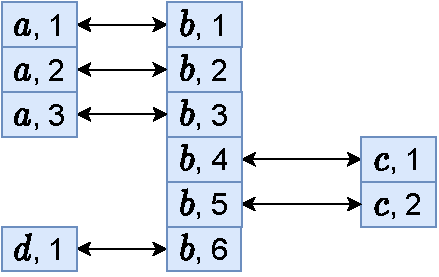
\includegraphics[scale=0.55]{diagrams/algorithm_k-lift_proof_simple_1.pdf}
    }%
    \subcaptionbox{
      A simple PN network $N_1$.
      \label{fig:algorithm:k-lift_proof_simple1:b}
    }%
      [.7\linewidth] {
      \centering
      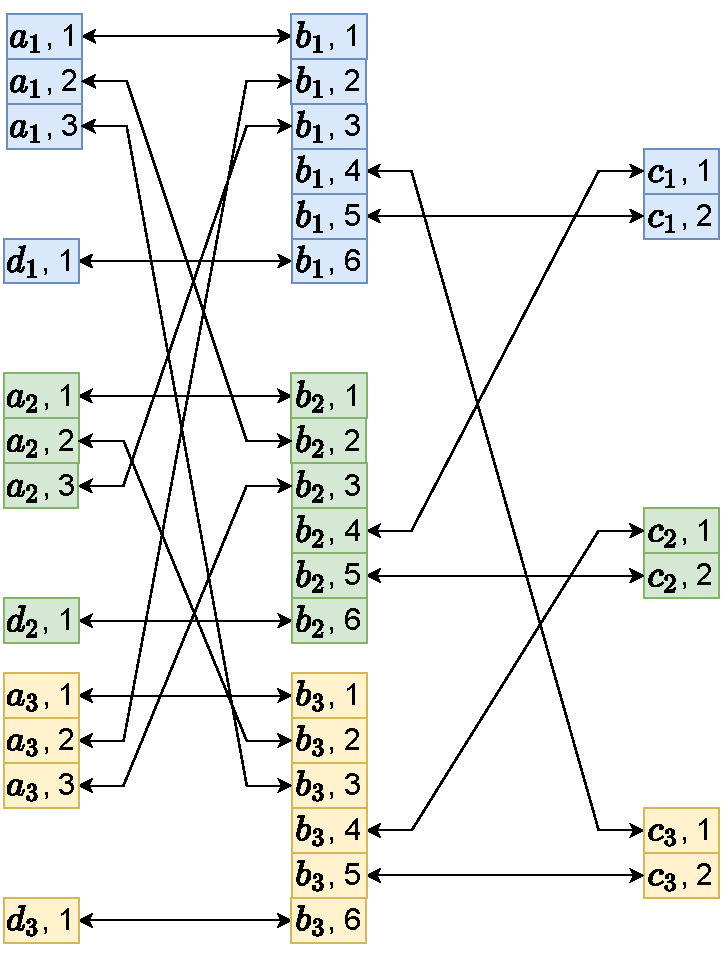
\includegraphics[scale=0.55]{diagrams/algorithm_k-lift_proof_simple_2.pdf}
    }
    \caption{The network $N_1$ is a 3-lift of the network $N_2$.
    }
    \label{fig:algorithm:k-lift_proof_simple1}
\end{figure}


\begin{lemma} \label{lem:lcl_unsolvability:from_multiple_to_simple}
    If an LCL problem $\Pi$ is not solvable in PN network $N_2$ with multiple connections, then it is also not solvable in simple PN network $N_1$ that is a lift of $N_2$.
\end{lemma}
\begin{proof}
    Let us assume that an LCL problem $\Pi$ is not solvable in PN network $N_2$ with multiple connections.
    Lemma \ref{lem:lcl_unsolvability:from_klift_to_simple} shows that there exists a k-lift $N_1$ of $N_2$ such that $N_1$ is a simple PN network.
    Lemma \ref{lem:lcl_unsolvability:from_multiple_to_lift} shows that the problem $\Pi$ is also not solvable in network $N_1$.
    Therefore, we deduce that the problem $\Pi$ is not solvable in simple PN network $N_1$ that is a lift of $N_2$.
\end{proof}


\subsection{From Finite to Infinite} \label{sec:algorithm:from_finite_to_infinite}
Our algorithm outputs a finite connected $(\Delta, \delta)$-biregular multigraph with cycles, but in the LCL formalism given in Section~\ref{sec:lcl_problems:biregular}, graphs are infinite $(\Delta, \delta)$-biregular trees.
Lemma~\ref{lem:lcl_unsolvability:from_multiple_to_simple} proves that unsolvability in PN network with multiple connections imply unsolvability in simple networks, but we also need to show how unsolvability in finite networks with cycles imply unsolvability in infinite tree networks.
We will prove this using graphs, and then from Lemma~\ref{lem:problem_unsolvability_in_graphs}, it immediately applies also to networks.

\begin{lemma} \label{lem:from_finite_to_infinite}
    If an LCL problem $\Pi$ is unsolvable in finite connected $(\Delta, \delta)$-biregular graph $G$ with cycles, then it is also unsolvable in some infinite $(\Delta, \delta)$-biregular tree $G'$.
\end{lemma}
\begin{proof}
    We construct an infinite $(\Delta, \delta)$-biregular tree $G'=(V', E')$ by \emph{unfolding} graph $G$.
    Let us fix a node $v \in V$.
    A non-backtracking walk is a walk that does not immediately visit a previous node at any point.
    %That is, an edge $\{u', v'\} \in G'$ \todo{Wait for better feedback on this}
    %We consider all possible non-backtracking walks from node $v$.
    %Two walks are adjacent, if one can be formed by adding a node to another.
    %For example $v-a-b-c-a$ and $v-a-b-c-a-b$ are considered as adjacent walks.
    Each node in $G'$ represents a non-backtracking walk in $G$ starting at node $v$.
    There is an edge between two nodes $u'$ and $v'$ in $G'$, if the walk presented by $u'$ can be obtained by the walk represented by $v'$ and one additional edge in $G$.
    %and adjacent non-backtracking walks are considered as adjacent nodes in $G'$.
    Graph $G$ has cycles, therefore there are infinite walks of infinite length.
    The walks are non-backtracking, therefore the constructed graph $G'$ must be $(\Delta, \delta)$-biregular.
    The graph $G'$ is a covering graph of $G$, because for each node $v' \in G'$, the 1-radius neighborhood of $v'$ is preserved.
    Using Lemma \ref{lem:lcl_unsolvability:from_multiple_to_lift}, we can conclude that the problem $\Pi$ must also be unsolvable in $G'$.
\end{proof}

%With Lemma \ref{lem:from_finite_to_infinite}, we can focus on finding finite connected $(\Delta, \delta)$-biregular graphs with cycles.

Now from Lemmas \ref{lem:problem_unsolvability_in_graphs}, \ref{lem:lcl_unsolvability:from_multiple_to_simple}, and \ref{lem:from_finite_to_infinite}, we can say that if Algorithm~\ref{alg:counterexample_finder} outputs a graph, then the problem is unsolvable, and the output graph is a proof of it.

\begin{figure}[H]
    \subcaptionbox{
     A (3,2)-biregular graph $G$
      \label{fig:algorithm:universal_cover:a}
    }%
      [.33\linewidth] {
      \centering
      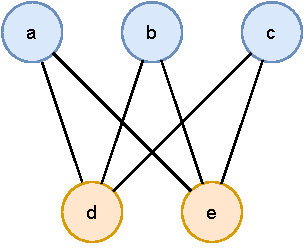
\includegraphics[scale=0.55]{diagrams/universal_cover_1.pdf}
    }%
    \hfill
    \subcaptionbox{
      An unfolding of graph $G$.
      Here the seed $v$ is node $d$ from graph $G$.
      \label{fig:algorithm:universal_cover:b}
    }%
      [.60\linewidth] {
      \centering
      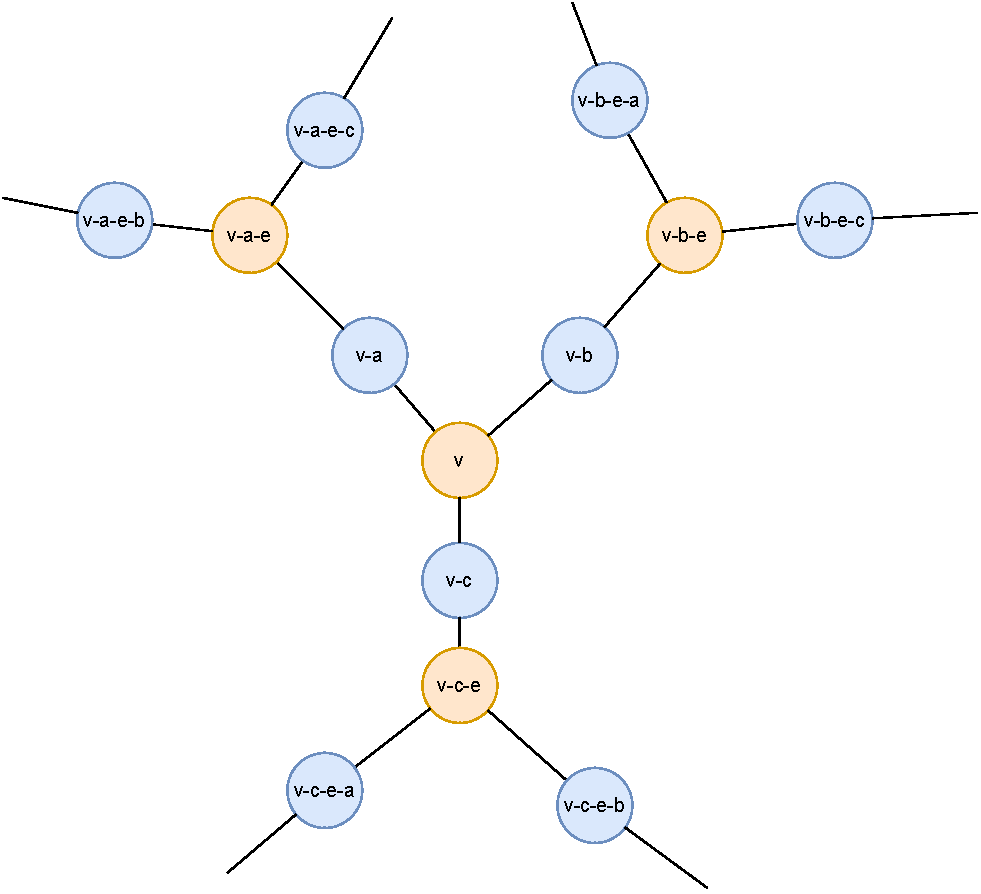
\includegraphics[scale=0.50]{diagrams/universal_cover_2.pdf}
    }
    \caption{A graph $G$ and its unfolding.
    }
    \label{fig:algorithm:universal_cover}
\end{figure}


\newpage
\subsection{From PN to LOCAL} \label{sec:algorithm:from_pn_to_local}

In this section we prove the following theorem:
\begin{theorem} \label{thm:algorithm:from_pn_to_local:lcl_unsolvability}
    If an LCL problem is unsolvable in the PN model, then the problem is also not solvable in constant time in the LOCAL model.
\end{theorem}

First, we introduce related lemmas, and at the end of this section, we prove Theorem~\ref{thm:algorithm:from_pn_to_local:lcl_unsolvability}.
The lemmas form a chain of implications shown in Figure~\ref{fig:proof_order:lcl_unsolvability}.
In the figure, there are two models we have to briefly introduce.
Both models are similar to the LOCAL and PN models in a sense that they are also message passing models.
We define them briefly as follows.

The first model is called \emph{order-invariant} (OI) \cite{DBLP:journals/siamcomp/NaorS95}.
The OI model can be thought as a LOCAL model with a restriction where each node can only compare the identifiers but not access their exact value.
In the model, the output of an algorithm does not change even if identifiers of nodes are changed as long as their relative order is preserved.

The second model called \emph{port numbering + orientation} (PO)~\cite{DBLP:conf/istcs/MayerNS95}.
In the PO model, ports are numbered like in the PN model, and additionally the edges have an orientation~\cite{DBLP:journals/dc/GoosHS17}.


\begin{figure}[H]
   \centering
   % https://tex.stackexchange.com/a/499577
   \begin{tikzpicture}[]
       \node (1) []             {$\mathcal{O}(1)$ LOCAL algorithm for $\Pi$ in general graphs};
       \node (2) [below = of 1] {$\mathcal{O}(1)$ LOCAL algorithm for $\Pi$ in trees};
       \node (3) [below = of 2] {$\mathcal{O}(1)$ OI algorithm for $\Pi$ in trees};
       \node (4) [below = of 3] {$\mathcal{O}(1)$ PO algorithm for $\Pi$ in trees};
       \draw[->] (1) -- (2) node [pos=0.5,left,font=\footnotesize] {Observation \ref{obs:algorithm:from_pn_to_local:o1_local_gen_imply_o1_local_trees}};
       \draw[->] (2) -- (3) node [pos=0.5,left,font=\footnotesize] {Lemma \ref{lem:algorithm:from_pn_to_local:o1_local_trees_imply_o1_oi_trees}};
       \draw[->] (3) -- (4) node [pos=0.5,left,font=\footnotesize] {Lemma \ref{lem:algorithm:from_pn_to_local:o1_oi_trees_imply_o1_po_trees}};
    \end{tikzpicture}
    \caption{Here are all the implications we show in this section.
    Each implication is a step towards showing Theorem \ref{thm:algorithm:from_pn_to_local:lcl_unsolvability}.
    %We use the notation $\exists\mathcal{O}(1)$ to denote the existence of a constant time algorithm.
    }
   \label{fig:proof_order:lcl_unsolvability}
\end{figure}

%%%% O(1) LOCAL in general graphs
% -> O(1) LOCAL in trees
\begin{observation} \label{obs:algorithm:from_pn_to_local:o1_local_gen_imply_o1_local_trees}
    If an LCL problem is solvable in constant time in the LOCAL model, then the problem is solvable in constant time in trees in the LOCAL model.
\end{observation}
\begin{proof}
    This is trivial, because general graphs contain the graph family of trees.
\end{proof}

%%%% O(1) LOCAL in trees
% -> O(1) OI in trees
\begin{lemma} \label{lem:algorithm:from_pn_to_local:o1_local_trees_imply_o1_oi_trees}
    If an LCL problem is solvable in constant time in trees in the LOCAL model, then the problem is solvable in constant time in trees in the OI model.
\end{lemma}
This has been proved for any fixed graph family in the work from Naor and Stockmeyer \cite[theorem 3.3]{DBLP:journals/siamcomp/NaorS95}.
The proof applies Ramsey theory to show that there exists a finite set $Y$ of identifiers such that for all $X_1, X_2 \subseteq Y$ with $|X_1| = |X_2| = s$, we have a constant time LOCAL algorithm giving identical results in any graph family whether we use identifiers $X_1$ or $X_2$.
It shows that the constant time LOCAL algorithm applied to identifiers from set $Y$ behaves like an OI algorithm.

%%%% O(1) OI in trees
% -> O(1) PO in trees
\begin{lemma} \label{lem:algorithm:from_pn_to_local:o1_oi_trees_imply_o1_po_trees}
    If an LCL problem is solvable in constant time in trees in the OI model, then the problem is solvable in constant time in trees in the PO model.
\end{lemma}
Suppose there is a $t$-time PO algorithm that solves an LCL problem.
The work from Göös et al.~\cite{DBLP:journals/dc/GoosHS17} shows that a PO algorithm can simulate an OI algorithm to solve the problem in $t$-time.


Now we prove Theorem \ref{thm:algorithm:from_pn_to_local:lcl_unsolvability}:
\begin{proof}[Proof of Theorem~\ref{thm:algorithm:from_pn_to_local:lcl_unsolvability}]
    Let us have an LCL problem $\Pi$ that is unsolvable in the PN model.
    In the LCL formalism, we have active and passive nodes.
    Let $N = (V, P, p)$ be an infinite ($\Delta, \delta$)-biregular tree network.
    Let $u, v \in V$ be distinct active nodes such that both $u$ and $v$ are adjacent to passive node $w\in V$.
    We can define an orientation between $u$ and $v$ by looking at the ports of node $w$.
    Let the port that connects from $w$ to $u$ be $(w, i)$, and let the port that connects from $w$ to $v$ be $(w, j)$.
    Port numbers $i$ and $j$ are distinct, therefore we can say that if $i < j$, then $u < v$.
    Otherwise, we say that $v < u$.
    Now, if we interpret the passive nodes as $\delta-uniform$ hyperedges, we can say that we have an orientation between any two adjacent nodes.
    Thus, when we work in the LCL formalism, we are actually already working in the PO model.
    Thus, $\Pi$ is also unsolvable in the PO model.

    Now, as shown in Figure \ref{fig:proof_order:lcl_unsolvability}, Observation~\ref{obs:algorithm:from_pn_to_local:o1_local_gen_imply_o1_local_trees}, and Lemmas~\ref{lem:algorithm:from_pn_to_local:o1_local_trees_imply_o1_oi_trees} and \ref{lem:algorithm:from_pn_to_local:o1_oi_trees_imply_o1_po_trees} form a chain of implications.
    This means that when there does not exist a constant time PO algorithm in trees for some LCL problem, there also does not exist a constant time LOCAL algorithm for the problem in general graphs.
    The problem $\Pi$ is unsolvable in the PN model and in the PO model.
    Therefore, problem $\Pi$ cannot be solved in constant time in the LOCAL model for general graphs.
\end{proof}



Now we have proved Theorem~\ref{thm:algorithm:from_pn_to_local:lcl_unsolvability}.
Therefore, the results from our algorithm now imply the problem is not solvable in constant time in the LOCAL model.
